\documentclass[letterpaper,landscape]{article}

%\usepackage[print]{pdfscreen}
\usepackage[screen,nopanel]{pdfscreen}
\margins{.5in}{.5in}{.5in}{.5in}
\screensize{6.25in}{8in}
\overlay{sunrise.jpg}
\notesname{Notes:}

% Switch mostly to Helvetica
\usepackage{helvet}
\usepackage{sectsty}
\allsectionsfont{\sffamily}

\begin{document}
\sffamily

\begin{slide}
\title{\resizebox{\textwidth}{!}{EtherIP Driver/Device Support}}
\author{kasemir@lanl.gov}
\date{Nov.\ 2003}
\color{section1}
\maketitle
\vfill
~~
\end{slide}

\begin{slide}
\section{EtherIP Driver/Device Support}
\begin{itemize}
\item Interfaces EPICS IOCs with Allen/Bradley ControlLogix 5000 PLCs
\item TCP-based Protocol: ControlNet-over-Ethernet, aka EtherNet/IP
      (IP=''Industrial Protocol'') or CIP (Control and Information Protocol)
\item Uses CIP extensions specific to ControlLogix 5000
\item Runs on vxWorks, RTEMS, Linux, Solaris, Win32\\
      (thanks to Stephanie Allison, SLAC)
\end{itemize}
\vfill
~~
\end{slide}

\begin{slide}
  \section{Driver/Device Interaction}
%% Trick: The minipage aligns top/center/bottom
%% by aligning the baseline.
%% With only the \includegraphics, that single line
%% would be the baseline and thus [t] == [b].
%% By adding zero-sized lines above and below \includegraphics,
%% we can actually use [t] and [b].
%% [From TUGBoat 17(1996)3 ]
  \begin{minipage}[t]{0.49\textwidth}
    \vspace{-\baselineskip}
    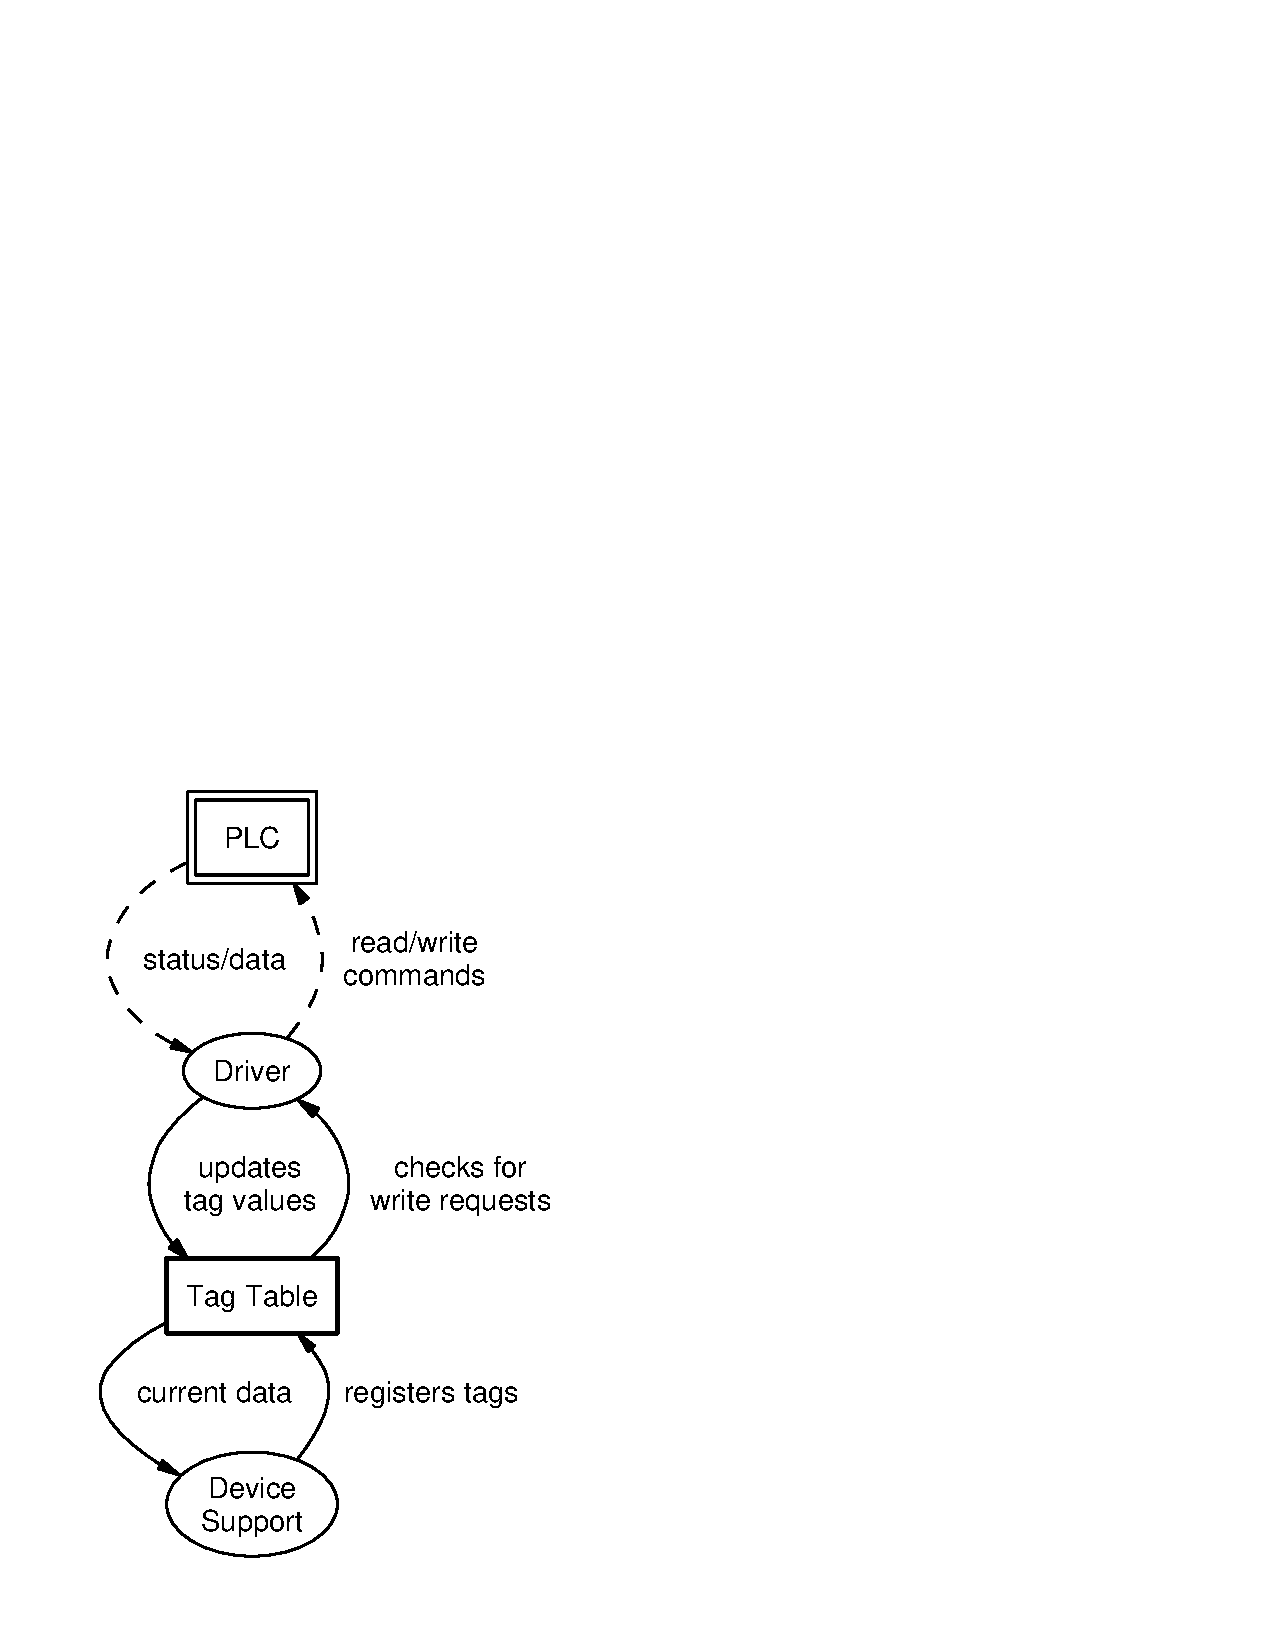
\includegraphics[height=\textheight]{driv_dev_rec}
    \par\vspace{0pt}
  \end{minipage}%
  \begin{minipage}[t]{0.49\textwidth}
    \begin{itemize}
    \item One driver thread per PLC
    \item Driver reads unless a tag is marked for 'write', which
      temporarily switches next cycle to write
    \item Device Support for AI/AO, BI/BO, MBBx, MBBxDirect, String,
      Waveform records
    \end{itemize}
    \vfill
    ~~
  \end{minipage}%
\end{slide}

\begin{slide}
\section{Tag Table Detail}
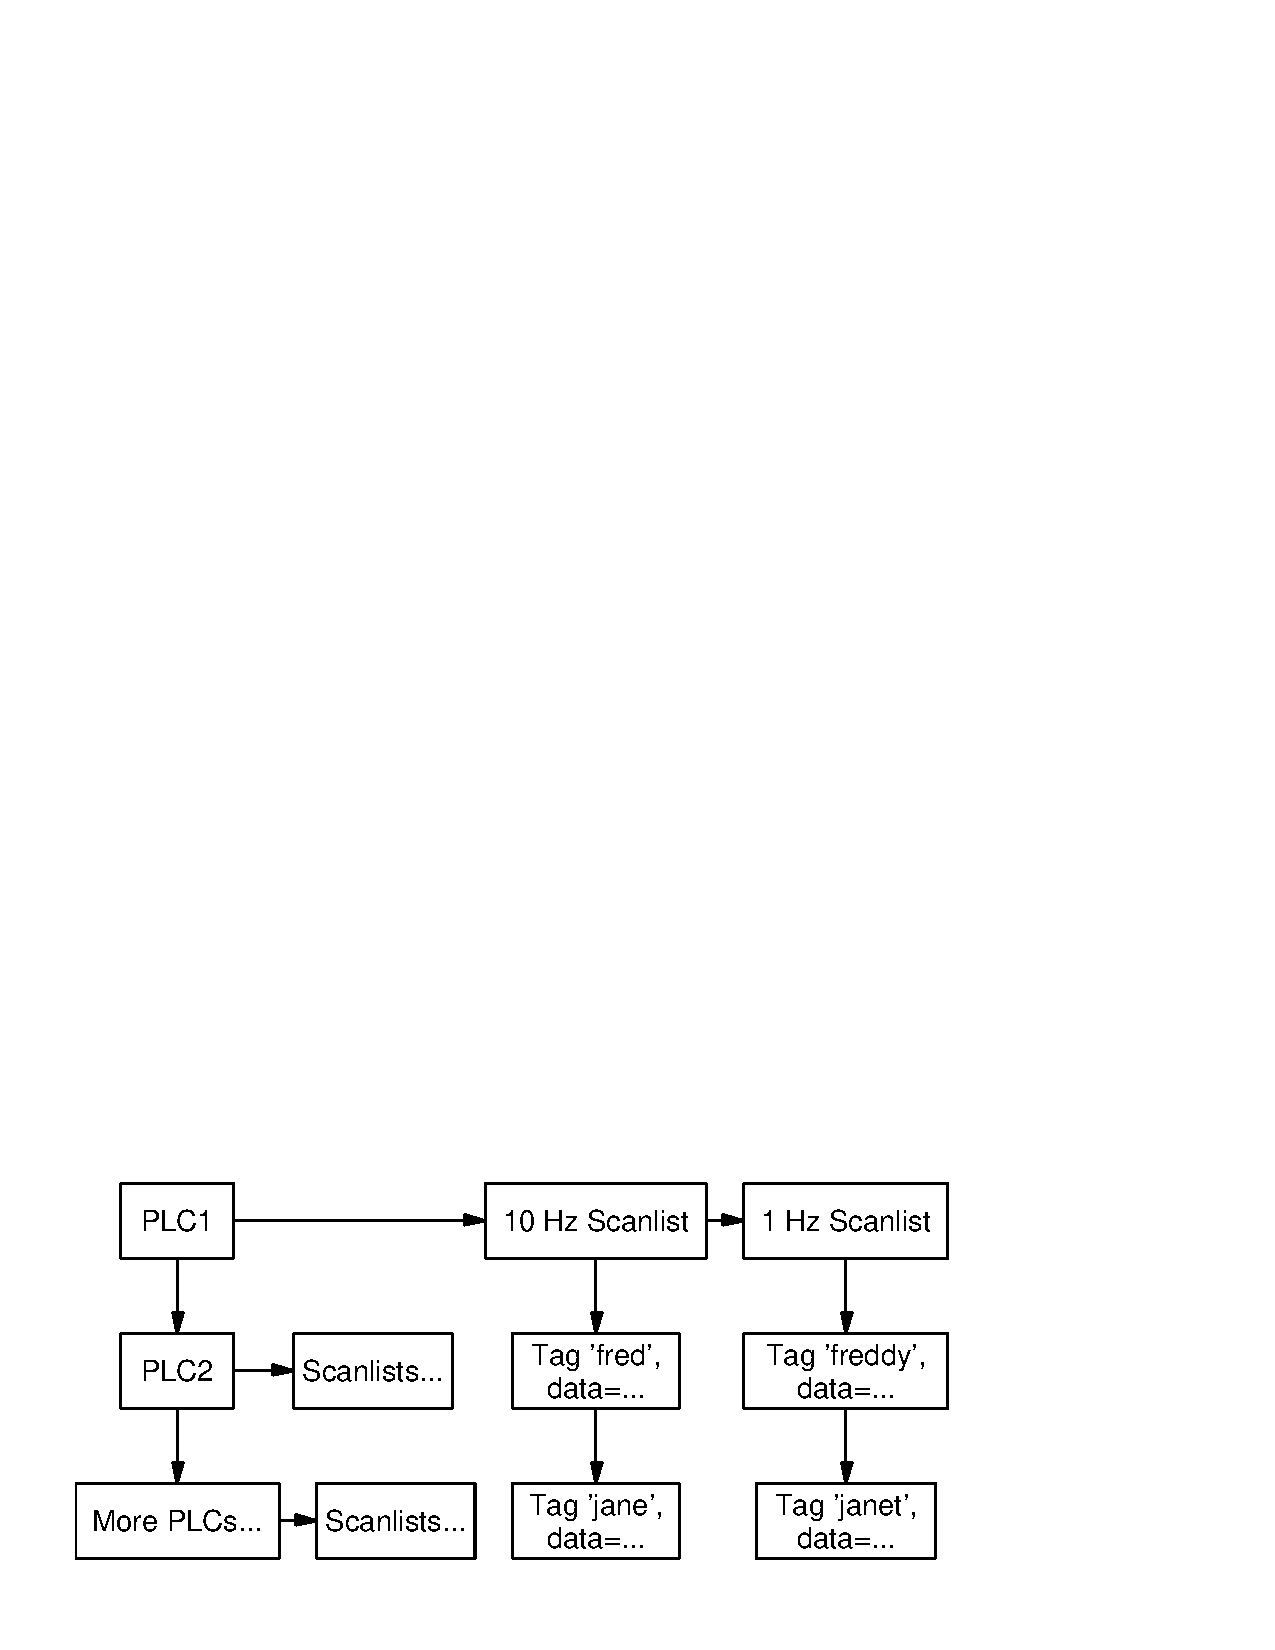
\includegraphics[width=0.8\textwidth]{tagtable}
\begin{itemize}
\item Driver task continually updates tags, their status, per-scanlist
  and per-PLC last \&\ total scan times 
\item Quite some code for combining as many reqeuests as possible into
  one xfer
\item Tags can be marked for 'write'
\item Device callbacks for 'new value' (SCAN=IO Intr, update ouput recs)
\end{itemize}
\end{slide}

\begin{slide}
\section{Usage 101}
\begin{itemize}
\item drvEtherIP\_define\_PLC(``PLC-ID'', ``IP'', slot-\#)
\item drvEtherIP\_initialize
\item DTYP="EtherIP", INP/OUT="\@PLC-ID tag\_x"
\item drvEtherIP\_help
\item drvEtherIP\_report (also via dbior)
\end{itemize}
\vfill
~~
\end{slide}

\begin{slide}
\section{Specialties}
\begin{itemize}
\item Runtime strcmp \& reparsing of INP/OUT
\item Analog record's VAL is used for floating-point tags, otherwise RVAL
\item Output records' tags are scanned, causing update \& process on
  change (device support hacks into VAL/RVAL and ten causes the
  SCAN=Passive records to be processed)
\item Special AI records for reading driver statistics
  (quite crummy to configure)
\end{itemize}
\vfill
~~
\end{slide}

\end{document}
                 
